\documentclass{article}
% 这里是导言区
%\usepackage{indentfirst}%缩进控制
\usepackage{listings}%插入代码
%\usepackage{mcode}
%ctex能够保证能够渲染英文
\usepackage{ctex}
\usepackage{textcomp}
\usepackage{graphicx}%插入图像
\usepackage{epstopdf}
\usepackage{amsmath}
\usepackage{graphicx}
\usepackage{subfigure}
\usepackage{geometry}%设置页边距
\usepackage{amssymb}
\usepackage{float}
\usepackage[level]{datetime} 
\makeatletter
\newcommand{\rmnum}[1]{\romannumeral #1}
\newcommand{\Rmnum}[1]{\expandafter\@slowromancap\romannumeral #1@}
\makeatother
% \renewcommand\thesection{\roman{subsection}}
%\newdateformat{ukdate}{\ordinaldate{\THEDAY} \monthname[\THEMONTH]

\geometry{a4paper,scale=0.75}


\lstset{
tabsize=4, %tab 空格数
frame=shadowbox, %把代码用带有阴影的框圈起来
rulesepcolor=\color{red!20!green!20!blue!20}, %代码块边框为淡青色
keywordstyle=\color{blue!90}\bfseries, %代码关键字的颜色为蓝色, 粗体
showstringspaces=false, %不显示代码字符串中间的空格标记
stringstyle=\ttfamily, %代码字符串的特殊格式
keepspaces=true, %
breakindent=22pt, %
numbers=left, %左侧显示行号
stepnumber=1, %
numberstyle=\tiny, %行号字体用小号
basicstyle=\footnotesize, %
showspaces=false, %
flexiblecolumns=true, %
breaklines=true, %对过长的代码自动换行
breakautoindent=true, %
breakindent=4em, %
aboveskip=1em, %代码块边框
}

\title{Chapter6}
\author{31202008881        \quad \quad \quad
          Bao Ze an}

\begin{document}
\setlength{\parindent}{2em}
\maketitle
\section*{6.1}
The system is a continous linear time invariant system,its controllability matrix:
\[
C=
\left[
\begin{array}{cccc}
B & AB & A^2B &A^3B
\end{array}
\right]   
=
\left[
    \begin{array}{ccc}
    1 & 0 & 0\\
    0 & 0 & -1\\
    0 & -1 & 3\\
    \end{array}
\right]
\]
$\rho(C)=3$,so the controllability matrix is full row rank, it is controllable.
its observability matrix:\\
\[
O=\left[
    \begin{array}{c}
        C\\
        CA\\
        CA^2\\
    \end{array}
\right]
=\left[
    \begin{array}{ccc}
    1 & 2 & 1\\
    -1 & -2 & -1\\
    1 & 2 & 1
    \end{array}
\right]   
\]
$\rho(O)=1 <3$, so the system is not observable.

\section*{6.2}
in the same way as in problem 6.1, but we can use the controllability index and observability index to 
simplify the calculation.
\[
C_\mu=
\left[
\begin{array}{cc}
B & AB
\end{array}
\right]   
=
\left[
    \begin{array}{cccc}
    0 & 1 & 1 & 0\\
    1 & 0 & 0 & 0\\
    0 & 0 & 2 & 0\\
    \end{array}
\right]
\]
the controllability matrix is full row rank,it is controllable.
\[
O=\left[
    \begin{array}{c}
        C\\
        CA\\
        CA^2\\
    \end{array}
\right]
=\left[
    \begin{array}{ccc}
    1 & 0 & 1\\
    0 & 3 & -1\\
    0 & -2 & 4
    \end{array}
\right]   
\]
$\rho(O)=3$, so the system is observable.

\section*{6.3}
it is not true,only if the matrix $A$ is nonsingular, it will be true.

\section*{6.4}
if the state equation is controllable ,so it must satisfy the PBH criterion.
\[
rank
\left[
    \begin{array}{ccc}
    A_{11}-\lambda I &A_{12} &B_1\\
    A_{21} & A_{22}-\lambda I & 0\\
    \end{array}
\right]=n   
\]
thus just means $[A_{21} A_{22}-SI]$ has full row rank.
$\iff {A_{22},A_{21}}$ controllable.

\section*{6.5}
\begin{figure}[hp]
    \centering
        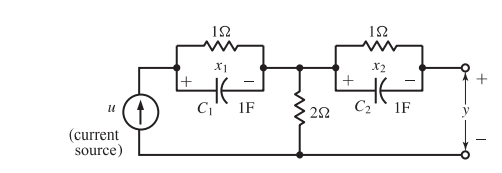
\includegraphics{png6.1.PNG}
        \end{figure}
Let $X_i$ be the voltage across the capacitor with capacitance.
\[
\left\{
\begin{aligned}
    &\dot{x_1}=u-x_1\\
    &\dot{x_2}=-x_2\\
    &y=2u-x_2\\
\end{aligned}    
\right.
\Rightarrow 
\]
\[
    \dot{x}
    \left[
        \begin{array}{cc}
            -1 & 0\\
            0 & -1\\
        \end{array}
    \right]x+
    \left[
        \begin{array}{c}
        1\\
        0
        \end{array}
    \right]u
\]
\[
    y=\left[
        \begin{array}{cc}
            0 & -1
        \end{array}
    \right]x+2u    
\]
The state equation is in Jordan-form,There are two jordan blocks, both with oreder 1, and 
associated  with eigenvalue -1, the entry of B corresponding to the second Jordan block is zero, 
so the state equation is not controllable.in the dual way, we can conclude it is not observable.

\section*{6.6}
\textbf{for the problem 6.1:}\\
The controllability matrix:
\[
C=
\left[
\begin{array}{ccc}
B & AB & A^2B 
\end{array}
\right]   
=
\left[
    \begin{array}{ccc}
    1 & 0 & 0\\
    0 & 0 & -1\\
    0 & -1 & 3\\
    \end{array}
\right]
\]
it is controllable,so its controllability index is $\mu=3$
because the system is not observable, so it is doesn't have a observability index.\\
\textbf{for problem 6.2}:
The controllability matrix:
\[
C=
\left[
\begin{array}{ccc}
B & AB & \cdots
\end{array}
\right]   
=
\left[
    \begin{array}{ccccc}
    0 & 1 & 1 & 0 & \cdots \\
    1 & 0 & 0 & 0 & \cdots \\
    0 & 0 & 2 & 0 & \cdots \\
    \end{array}
\right]
\]
because $Ab_2=[0\ 0\ 0]'$, so the controllability indices are 2,1,so the controllability index is $\mu=max(\mu_1,\mu_2)=2$
The system is observable,and the matrix C's row rank is 1,so the observability index is $v=3$.

\section*{6.7}
The controllability index is 1.

\section*{6.8}
The controllability matrix is:\\
\[
    C=
    \left[
    \begin{array}{cc}
    B & AB
    \end{array}
    \right]   
    =
    \left[
        \begin{array}{cc}
        1 & 3\\
        0 & 3\\
        \end{array}
    \right]  
\]
$\rho(C)=1$, take a canonical decomposition
\[
P^{-1}=
\left[
    \begin{array}{cc}
        1 & 0\\
        1 & 1
    \end{array}
\right]
P=
\left[
    \begin{array}{cc}
        1 & 0\\
        -1 & 1
    \end{array}
\right]
\]
\[
PAP^{-1}=
\left[
    \begin{array}{cc}
        3 & 4\\
        0 & -5
    \end{array}
\right]
PB=
\left[
    \begin{array}{c}
        1\\
        0 
    \end{array}
\right]
CP^{-1}=
\left[
    \begin{array}{cc}
        2 & 1\\
    \end{array}
\right]
\]
\[
\begin{split}
\dot{\bar{x}}=PAP^{-1}\bar{x}+PBu\\
y=CP^{-1}\bar{x}
\end{split}   
\]
so the reduced controllable equation is:
\[
\begin{split}
    \dot{\bar{x_c}}=3\bar{x_c}+u\\
    y=2\bar{x_c}
\end{split}
\]
The reduced equation is observable.

\section*{6.9}
The controllable and observable equation is $y=2u$,none of the states are controllable and observable.

\section*{6.10}
The state equation is in Jordan-form.
using the corollary 6.8, we can conclude that $x_3$ is not controllable, we rearrange the equation as:
\[
\left[
    \begin{array}{c}
        \dot{x_1}\\
        \dot{x_2}\\
        \dot{x_4}\\
        \dot{x_5}\\
        \dot{x_3}
    \end{array}
\right]=
\left[
    \begin{array}{ccccc}
    \lambda_1 & 1 & 0 & 0 & 0 \\
    0 & \lambda_1 & 0 & 0 & 1 \\
    0 & 0 & \lambda_2 & 1 & 0 \\
    0 & 0 & 0 & \lambda_2 & 0 \\
    0 & 0 & 0 & 0 & \lambda_1
    \end{array}
\right]
\left[
    \begin{array}{c}
        x_1\\
        x_2\\
        x_4\\
        x_5\\
        x_3
    \end{array}
\right]+
\left[
    \begin{array}{c}
        0\\
        1\\
        0\\
        1\\
        0
    \end{array}
\right]u
\] 
\[
y=
\left[
    \begin{array}{ccccc}
        0 & 1 & 0 & 1 & 1
    \end{array}
\right]x
\]
thus  we can reduce the equation as:
\[
\left[
    \begin{array}{c}
        \dot{x_1}\\
        \dot{x_2}\\
        \dot{x_4}\\
        \dot{x_5}\\
    \end{array}
\right]=
\left[
    \begin{array}{cccc}
        \lambda_1 & 1 & 0 & 0\\
        0 & \lambda_1 & 0 & 0\\
        0 & 0 & \lambda_2 & 1\\
        0 & 0 & 0 & \lambda_2
    \end{array}
\right]
\left[
    \begin{array}{c}
        x_1\\
        x_2\\
        x_4\\
        x_5\\
    \end{array}
\right]+
\left[
    \begin{array}{c}
        0\\
        1\\
        0\\
        1\\
    \end{array}
\right]u
\] 
\[
y=
\left[
    \begin{array}{cccc}
        0 & 1 & 0 & 1 
    \end{array}
\right]x
\]
from the output equation,we can easily find that state $x_1$ and $x_4$ is not observable.
\[
\left[
    \begin{array}{c}
        \dot{x_2}\\
        \dot{x_5}\\
        \dot{x_1}\\
        \dot{x_4}\\
    \end{array}
\right]=
\left[
    \begin{array}{cccc}
        \lambda_1 & 0 & 0 & 0\\
        0 & \lambda_2 & 0 & 0\\
        1 & 0 & \lambda_1 & 0\\
        0 & 1 & 0 & \lambda_2
    \end{array}
\right]
\left[
    \begin{array}{c}
        x_2\\
        x_5\\
        x_1\\
        x_4\\
    \end{array}
\right]+
\left[
    \begin{array}{c}
        1\\
        1\\
        0\\
        0\\
    \end{array}
\right]u
\] 
\[
y=
\left[
    \begin{array}{cccc}
        1 & 1 & 0 & 0
    \end{array}
\right]x
\]
so the controllable and observable equation is:
\[
\dot{x}=
\left[
    \begin{array}{cc}
        \lambda_1 & 0\\
        0 & \lambda_2
    \end{array}
\right]x+
\left[
    \begin{array}{c}
        1\\
        1
    \end{array}
\right]u
\]
\[
y=
\left[
    \begin{array}{cc}
        1 & 1
    \end{array}
\right]x    
\]

\section*{6.11}
Select an arbitrary $Q_2$ such that $[Q_1\ Q_2]$ is nonsingular,define 
\[
\left[
    \begin{array}{c}
    P_1\\
    P_2
    \end{array}
\right]=
\left[
    \begin{array}{cc}
        Q_1 & Q_2
    \end{array}
\right]^{-1}
\]
thus
\[
\left[
    \begin{array}{c}
    P_1\\
    P_2
    \end{array}
\right]
\left[
    \begin{array}{cc}
        Q_1 & Q_2
    \end{array}
\right]=
\left[
    \begin{array}{cc}
        P_1Q_1 & P_1Q_2\\
        P_2Q_1 & P_2Q_2
    \end{array}
\right]
=
\left[
    \begin{array}{cc}
        I_{n_1} & 0\\
        0 & I_{n-n_1}
    \end{array}
\right]
\]
we know $P_2Q_1=0$ and $Q_1$ consists of all linearly indepedent columns of 
\[
\left[
    \begin{array}{cccc}
        B & AB &\cdots & A^{n-1}B
    \end{array}
\right]    
\]
we can conclude that $P_2B=0$ and $P_2AQ_1=0$,let consider the transformation 
\[
\dot{x}=
\left[
    \begin{array}{c}
        P_1\\
        p_2
    \end{array}
\right]x    
\]
\[
\bar{A}=
\left[
    \begin{array}{c}
        P_1\\
        P_2
    \end{array}
\right]A
\left[
    \begin{array}{cc}
        Q_1 &Q_2
    \end{array}
\right]=
\left[
    \begin{array}{cc}
        P_1AQ_1 & P_1AQ_2\\
        P_2AQ_1 & P_2AQ_2\\
    \end{array}
\right]
\]
\[
\bar{B}=\left[
\begin{array}{c}
    P_1\\
    P_2
\end{array}
\right]B=
\left[
    \begin{array}{c}
        P_1B\\
        P_2B
    \end{array}
\right]    
\]
\[
\bar{C}=C
\left[
    \begin{array}{cc}
        Q_1 & Q_2
    \end{array}
\right]=
\left[
    \begin{array}{cc}
        CQ_1 & CQ_2
    \end{array}
\right]
\]
Because $P_2B=0$ and $P_2AQ_1=0$, the equation can be reduced to the controllable equation:
\[
    \begin{split}
    \dot{\bar{x_1}}=P_1AQ_1\bar{x_1}+P_1Bu\\
    y=CQ_1\bar{x_1}+Du
    \end{split}
\] 
\section*{6.12}
Let $P$ be a unit-matrix,take elementary row operation to tranformate $Q_1$ inducto
\[
PQ_1=
\left[
    \begin{array}{c}
        I_{n_1}\\
        0
    \end{array}
\right]    
\]
The first $n_1$ row of $P$ is $P_1$.
\section*{6.13}
consider the n-dimensional state equation:
\[
\begin{split}
    \dot{x}=Ax+Bu\\
    y=Cx+Du\\
\end{split}    
\]
The rank of its observability matrix is assumed to be $n_2<n$.Let $P_2$ be an $n_2xn$ matrix whose rows are any
$n_2$ linearly indepedent rows of the observability matrix .Let $Q_2$ be an $nxn_2$ matrix such that $P_2Q_2=I_{n2}$
where $I_{n2}$ is the unit matrix of order $n_2$,\\
the following $n_2$-dimensional state equation\\ 
\[
\left\{
\begin{aligned}
    &\dot{\bar{x_2}}=P_2AQ_2\bar{x_2}+P_2Bu\\
    &\bar{y}=CQ_2\bar{x_2}+Du
\end{aligned}
\right.   
\]
is observable and has the same transfer matrix as the original state equation.

\section*{6.14}
There are three Jordan blocks,with order 2,1 and 1 associated with 2 and two Jordan blocks, with order 2,1 associated with 1.
The entry of B corresponding to the last row of the the first three block are 
$[2,1,1],[1,1,1]\ and\ [3,2,1]$, and they are linearly indepedent .The entry of B corresponding to the last row of the second two Jordan block are $[1,0,1]\ and\ [1,0,0]$,they are also linearly indepedent ,so the Jordan-form state equation is controllable.\\
unforately,The entry of C corresponding to the first column of the first three Jordan block are $[2,1,0]' ,[1,1,1]'\ and\ [3,2,1]'$, but they are linearly depedent.
so the Jordan-form state equation is not observable.

\section*{6.15}
if required Jordan-form state equation is controllable,only if the $[b_{21}\ b_{22}],[b_{41}\ b_{42}]\ and\ [b_{51}\ b_{52}]$ is linearly indepedent, this is obviously impossible.
so it is not impossible to find a set of $b_{ij}$ such that the state equation is controllable.but, we can find a set of $c_{ij}$ such that the state equation is observable,just make the 
\[
\left[
    \begin{array}{ccc}
        c_{11} & c_{13} & c_{15}\\
        c_{21} & c_{23} & c_{25}\\
        c_{31} & c_{33} & c_{35}
    \end{array}
\right]    
\]
is nonsingular.

\section*{6.16}
Take an equivalence transformation ,$\bar{x}=Px$\\
\[
P=
\left[
    \begin{array}{ccccc}
     1 & 0 & 0 & 0 & 0\\
     0 & 0.5 &-0.5j & 0 & 0\\
     0 & 0.5 &0.5j & 0 & 0\\
     0 & 0 & 0 & 0.5 & -0.5j\\
     0 & 0 & 0 &0.5 &0.5j
    \end{array}
\right]    
\]
\[
\bar{A}=PAP^{-1}=
\left[
    \begin{array}{ccccc}
        \lambda_1 & 0 & 0 &0 & 0\\
        0 & \alpha_1+j\beta_1 & 0 & 0 & 0\\
        0 & 0 & \alpha_1-j\beta_1 & 0 & 0\\
        0 & 0 & 0 & \alpha_2+j\beta_2 & 0\\
        0 & 0 & 0 & 0 & \alpha_2-j\beta_2
    \end{array}
\right]
\]
\[
\bar{B}=PB=
\left[
    \begin{array}{c}
        b_1\\
        0.5b_{11}-0.5b_{12}j\\
        0.5b_{11}+0.5b_{12}j\\
        0.5b_{21}-0.5b_{22}j\\
        0.5b_{21}+0.5b_{22}j
    \end{array}
\right]    
\]
\[
\bar{C}=CP^{-1}
=\left[
    \begin{array}{ccccc}
        c_1 & c_{11}+jc_{12} & c_{11}-jc_{12} & c_{21}+jc_{22} & c_{21}-jc_{22}
    \end{array}
\right]    
\]
The equivalence transformation doesn't change the controllability and observability.
for:
\[
\begin{split}
\dot{\bar{x}}=\bar{A}\bar{x}+\bar{B}u\\
y=\dot{C}\bar{x}    
\end{split}
\]
it is controllable $\iff b_1 \neq 0,b_{i1} \neq 0$ or $ b_{i2} \neq 0 $ (for i=1,2)\\
it is observable $\iff c_1 \neq 0,c_{i1} \neq 0$ or $ c_{i2} \neq 0 $ (for i=1,2)

\section*{6.17}
Let $x_1,x_2$ be the states and $x_3$ can be expressed by $x_1,x_2$,so the two-dimensional state equation is :
\[
\left\{
\begin{aligned}
    &y=-x_1-x_2\\
    &\dot{x_2}=-3(\dot{x_1}+\dot{x_2})\\
    &\frac{u+x_1}{2}+2\dot{x_1}=\dot{x_2}
\end{aligned}    
\right.    
\]
\[
    \left[
        \begin{array}{c}
            \dot{x_1}\\
            \dot{x_2}
        \end{array}
    \right]=
    \left[
        \begin{array}{cc}
            -\frac{11}{2} & 0\\
            \frac{3}{22} & 0
        \end{array}
    \right]
    \left[
        \begin{array}{c}
            x_1\\
            x_2
        \end{array}
    \right]+
    \left[
        \begin{array}{c}
            -\frac{2}{11}\\
            \frac{3}{22}
        \end{array}
    \right]u    
\]
\[
y=\left[
    \begin{array}{cc}
        -1 & -1
    \end{array}
\right]
\left[
    \begin{array}{c}
        x_1\\
        x_2
    \end{array}
\right]    
\]
The controllability matrix:
\[
C=\left[
    \begin{array}{ccc}
        -\frac{2}{11} & -\frac{2}{11}\times (-\frac{2}{11})\\
        \frac{3}{22} & \frac{3}{22} \times (-\frac{2}{11})
    \end{array}
\right]    
\]
it is easily to see that $\rho(c)=1<2$,it is not controllable.
The three-dimensional state equations:
from $x_3=-x_1-x_2$, we can get $\dot{x_3}=-\dot{x_1}-\dot{x_2}=\frac{1}{22}x_1+\frac{1}{22}u$
\[
    \left[
        \begin{array}{c}
            \dot{x_1}\\
            \dot{x_2}\\
            \dot{x_3}
        \end{array}
    \right]=
    \left[
        \begin{array}{ccc}
            -\frac{11}{2} & 0 & 0\\
            \frac{3}{22} & 0 & 0\\
            \frac{1}{22} & 0 & 0\\
        \end{array}
    \right]
    \left[
        \begin{array}{c}
            x_1\\
            x_2\\
            x_3
        \end{array}
    \right]+
    \left[
        \begin{array}{c}
            -\frac{2}{11}\\
            \frac{3}{22}\\
            \frac{1}{22}
        \end{array}
    \right]u    
\]
\[
y=\left[
    \begin{array}{ccc}
        0 & 0 & 1
    \end{array}
\right]
\left[
    \begin{array}{c}
        x_1\\
        x_2\\
        x_3
    \end{array}
\right]    
\]


\section*{6.18}
%一定要注意电路里的源是电流源还是电压源
%这对树(tree)的选取至关重要。
\par
\centerline{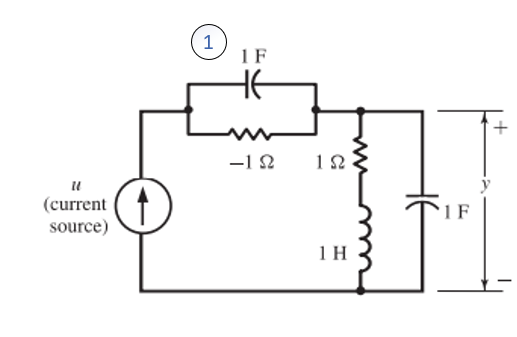
\includegraphics{a2.191.PNG}}
\centerline
\par
The voltage across the 1-F capacitor number 1 is assigned $x_1$,then its current is $\hat{x_1}$,the voltage across the other 1-F capacitor is assigned
$x_2$,then its current is $\hat{x_2}$,the current through the 1-H inductor is assigned as $x_3$,
then its voltage is $\hat{x_3}$\\
According to the Kirchhoff's current law and Kirchhoff's voltage law,we can get the equation following:
\[\left\{    
\begin{aligned}
&\dot{x_1}=x_1+u&\\
&\dot{x_2}=-x_3+u&\\
&\dot{x_3}=x_2-x_3&\\
&y=x_2&\\
\end{aligned}
\right.
\]
Rewrite them in matrix form:
\begin{equation*}       %开始数学环境
    \left[                %左括号
    \begin{array}{c}   %该矩阵一共3列,每一列都居中放置
    \dot{x_1} \\  %第一行元素
    \dot{x_2} \\  %第二行元素
    \dot{x_3} \\
    \end{array}
    \right]=      %右括号
    \left[                %左括号
    \begin{array}{ccc}   %该矩阵一共3列,每一列都居中放置
    -1 & 0 & 0\\
    0 & 0 & -1\\
    0 & 1 & -1\\    
    \end{array}
    \right]
    \left[                %左括号
    \begin{array}{c}   %该矩阵一共3列,每一列都居中放置
    x_1 \\  %第一行元素
    x_2 \\  %第二行元素
    x_3 \\
    \end{array}
    \right]+
    \left[                %左括号
    \begin{array}{c}   %该矩阵一共3列,每一列都居中放置
    1 \\  %第一行元素
    1 \\  %第二行元素
    0 \\
    \end{array}
    \right]u               
\end{equation*}

\begin{equation*}
y=\left[
\begin{array}{ccc}
0 & 1 & 0\\
\end{array}
\right]
\left[
\begin{array}{c}
x_1 \\  %第一行元素
x_2 \\  %第二行元素
x_3 \\
\end{array}
\right]
\end{equation*}

its controllability matrix:
\[
C=
\left[
\begin{array}{cccc}
B & AB & A^2B
\end{array}
\right]   
=
\left[
    \begin{array}{ccc}
    1 & -1 & 1\\
    1 & 0 & -1\\
    0 & 1 & -1\\
    \end{array}
\right]
\]
$\rho(C)=3$,it is have full row rank,so the state equation is controllable.
its controllability matrix is:
\[
O=\left[
    \begin{array}{c}
        C\\
        CA\\
        CA^2\\
    \end{array}
\right]
=\left[
    \begin{array}{ccc}
    0 & 1 & 0\\
    0 & 0 & -1\\
    0 & -1 & 1
    \end{array}
\right]   
\]
$\rho(O)=2<3$,so the state equation is not observable.
The RC loop doesn't have influence on the current source,the RC loop can be regarded as 
a wire, so the response of $x_1$ will not affect the output of the network.so the network is not observable.  

\section*{6.19}
Let $u(t)$ is piecewise constant,that is to say,the input changes values only at discrete-time instants.
we get the discrete-time equation without the approximation:
\[
\begin{aligned}
x[k+1]=A_dx[k]+B_du[k]\\
y[k]=C_dx[k]+D_du[k]\\
\end{aligned}    
\]
where $A_d=e^{AT},B_d=(\int_{0}^{T}e^{A\tau}d\tau)B,C_d=C,D_d=D$
when $T=1$:
\[
A_d=e^{A}=
\left[
\begin{array}{cc}
e^{-1}(cos1+sin1) & e^{-1}sin1 \\
-2e^{-1}sin1 & e^{-1}(cos1-sin1)\\
\end{array}
\right]
\]
%不要老是用calculate表示计算这个英文,要学会使用compute这个单词
Because A is nonsingular, so we can compute the
\[
B_d=A^{-1}(A_d-I)B=
\left[
\begin{array}{c}
1.0491\\
-0.1821
\end{array}
\right]    
\]
\[
C_d=C=
\left[
\begin{array}{cc}
2 &3\\
\end{array}
\right] 
\]
thus the discrete-time equation:
\[
x[k+1]=
\left[
\begin{array}{cc}
e^{-1}(cos1+sin1) & e^{-1}sin1 \\
-2e^{-1}sin1 & e^{-1}(cos1-sin1)\\
\end{array}
\right]x[k]+
\left[
\begin{array}{c}
1.0491\\
-0.1821
\end{array}
\right]u[k]
\]
\[
y[k]=
\left[
\begin{array}{cc}
2 &3\\
\end{array}
\right]x[k]
\]
in the same way,for $T=\pi$:
\[
x[k+1]=
\left[
\begin{array}{cc}
-0.0432 & 0 \\
0 & -0.0432\\
\end{array}
\right]x[k]+
\left[
\begin{array}{c}
1.5648\\
-1.0432
\end{array}
\right]u[k]
\]
\[
y[k]=
\left[
\begin{array}{cc}
2 &3\\
\end{array}
\right]x[k]
\]
for the original state equation(continous),its controllability matrix:
\[
    C=
    \left[
    \begin{array}{cc}
    B & AB
    \end{array}
    \right]   
    =
    \left[
        \begin{array}{cc}
        1 & 1\\
        1 & -4\\
        \end{array}
    \right]  
\]
$\rho(C)=2$,so the continous system is controllable.
its observability matrix:
\[
    O=
    \left[
    \begin{array}{c}
    C \\
    CA \\
    \end{array}
    \right]   
    =
    \left[
        \begin{array}{cc}
        2 & 3\\
        -6 & -4\\
        \end{array}
    \right]  
\]
$\rho(O)=2$,so the continous system is observable.\\
its eigenvalues are:$\lambda_1=-1+i,\lambda_2=-1-i$\\
the sufficient condition:$\vert{Im[\lambda_1-\lambda_2]}\vert \neq \frac{2\pi m}{T}$
thus to say:$2 \neq \frac{2\pi m}{T}$,$T \neq \pi m$\\
for sampling period T=1:\\
it satisfy the condition, so it is controllable and observable.\\
for sampling period T=$\pi$:\\
it doesn't satisfy the condition,and it is a SISO problem,so it is also a necessary condition.so it is not controllable and observable.

\section*{6.20}
This is a LTV system,
using the theorem 6.12,$M_0(t)=B(t)$,$M_1(t)=-A(t)M_0(t)+\frac{\mathrm{d}}{\mathrm{d}t}M_0(t)$\\
we have:
\[
\left[
    \begin{array}{cc}
    M_0(t) & M_1(t)        
    \end{array}
\right]=
\left[
    \begin{array}{cc}
    0 & -1\\
    1 & -t    
    \end{array}
\right] 
\]
for any t,$rank[M_0(t)\ M_1(t)]=2$,so the state eqution is controllable.\\
in the same way,$N_0(t)=C(t)$, and $N_1(t)=N_0(t)A(t)+\frac{\mathrm{d}}{\mathrm{d}t}N_0(t)$
because the theorem 6.12 is not a necessary and sufficient condition, but we can extend the therom 6.o12
\[
\left[
    \begin{array}{c}
    N_0(t)\\
    N_1(t)\\
    N_2(t)\\
    \vdots        
    \end{array}
\right]=
\left[
    \begin{array}{cc}
    0 & 1\\
    0 & t \\
    0 & t^2\\
    \vdots   
    \end{array}
\right] 
\]
there doesn't exist a $t$ make the 
\[
rank
\left[
    \begin{array}{c}
    N_0(t)\\
    N_1(t)\\
    \vdots       
    \end{array}
\right]=2
\]
so the system is not observable.using the theorem 6.o11,we can also check the observability.
we can compute the solution of $x_1(t),x_2(t)$\\
\[
\left\{
    \begin{aligned}
    & x_1(t)=\int_0^tx_2(0)e^{0.5t^{2}}dt +x_1(0)\\
    & x_2(t)=x_2(0)e^{0.5t^2}\\
    \end{aligned}
\right.    
\]
let 
\[
\left[
    \begin{aligned}
        x_1(0)\\
        x_2(0)
    \end{aligned}
\right]=
\left[
    \begin{aligned}
        0\\
        1
    \end{aligned}
\right]
or
\left[
    \begin{aligned}
        x_1(0)\\
        x_2(0)
    \end{aligned}
\right]=
\left[
    \begin{aligned}
        1\\
        0
    \end{aligned}
\right]
\]
we can get the fundamental matrix:
\[
\left[
    \begin{array}{cc}
        1 & \int_0^t e^{0.5t^2}dt\\
        0 & e^{0.5t^2}
    \end{array}
\right]    
\]
so,from the fundamental matrix ,we can easily get the state transition matrix:
\[
\phi(t,t_0)=
\left[
    \begin{array}{cc}
        1 & e^{-0.5t_0^2}\int_0^t e^{0.5\tau^2}d \tau\\
        0 & e^{0.5(t^2-t_0^2)}
    \end{array}
\right]  
\]  
we can get:\\
\[
C\phi(\tau,t_0)=
\left[
    \begin{array}{cc}
    0 & e^{0.5(\tau^2-t_0^2)}
    \end{array}
\right]   
\]
so the 
\[W_o(t_0,t_1)=
\int_{t_0}^{t_1}
\left[
    \begin{array}{cc}
        0 & 0\\
        0 & e^{\tau^2-t_0^2}
    \end{array}
\right]d\tau
\]
it is singular,so it is not observable.

\section*{6.21}
%还是老老实实的用第一种发方法求解W矩阵吧
This is a LTV system,
using the theorem 6.12,$M_0(t)=B(t)$,$M_1(t)=-A(t)M_0(t)+\frac{\mathrm{d}}{\mathrm{d}t}M_0(t)$\\
we have:
\[
\left[
    \begin{array}{cc}
    M_0(t) & M_1(t)        
    \end{array}
\right]=
\left[
    \begin{array}{cc}
    1 & 0\\
    e^{-t} & 0
    \end{array}
\right] 
\]
for this sufficient condition, we can't check its controllability.
its state transition matrix is:
\[
\Phi(t,t_0)=
\left[
    \begin{array}{cc}
        1 & 0\\
        0 & e^{-(t-t_0)}
    \end{array}
\right]    
\]
we can get:
\[
\Phi(t_1,\tau)B(\tau)=
\left[
    \begin{array}{c}
        1\\
        e^{-t_1}
    \end{array}
\right]    
\]
\[
W_c(t_0,t_1)=
\int_{t_0}^{t_1}
\left[
    \begin{array}{cc}
        1 & e^{-t_1}\\
        e^{-t_1} & e^{-2t_1}
    \end{array}
\right]d\tau
=\left[
    \begin{array}{cc}
        t_1-t_0 & e^{-t_1}(t_1-t_0)\\
        e^{-t_1}(t_1-t_0) & e^{-2t_1}(t_1-t_0)
    \end{array}
\right]
\]
the determinant of $W_c(t_0,t_1)$ is zero,so it is singular, so the state euqation is not controllable.
in the same way,$N_0(t)=C(t)$, and $N_1(t)=N_0(t)A(t)+\frac{\mathrm{d}}{\mathrm{d}t}N_0(t)$
\[
\left[
    \begin{array}{c}
    N_0(t)\\
    N_1(t)\\      
    \end{array}
\right]=
\left[
    \begin{array}{cc}
    0 & e^{-t}\\
    0 & -2e^{-t} \\
    \end{array}
\right] 
\]
there doesn't exist a $t$ make the 
\[
rank
\left[
    \begin{array}{c}
    N_0(t)\\
    N_1(t)\\      
    \end{array}
\right]=2
\]
theorem 6.o12 can not check the observability.
so we use the theorem 6.o11,
\[
C(\tau)\Phi(\tau,t_0)=
\left[
    \begin{array}{cc}
        0 & e^{-(2\tau-t_0)}
    \end{array}
\right]
\]
\[
W_o(t_0,t_1)=
\int_{t_0}^{t_1}
\left[
    \begin{array}{cc}
        0 & 0\\
        0 & e^{-4\tau-2t_0}
    \end{array}
\right]d\tau
\]
it is easily to find the $W_o(t_0,t_1)$ is singular,so the state equation is not observable. 

\section*{6.22}
Let X(t) be a fundamental matrix of $\dot{x}=A(t)x$
we know $X^{-1}(t)X(t)=I$,taking differentiation on both sides of the equation,we can get 
%这里的\mathrm的作用是将公式中的斜体变成罗马体,也就是正体
\[
    \frac{\mathrm{d}}{\mathrm{d}t}X^{-1}(t)=-X^{-1}(t)A(t) 
\]
in the same way,we suppose:
\[
\dot{x(t)}=-A(t)'x(t)    
\]
Let $X_1(t)$ be a fundamental matrix of $\dot{x(t)}=-A'(t)x(t)$
we can easily find that 
$$
\begin{aligned}
\frac{\mathrm{d}}{\mathrm{d}t}X_{1}(t)=-A'(t)X_{1}(t)\\
\frac{\mathrm{d}}{\mathrm{d}t}X'_{1}(t)=-X'_{1}(t)A(t)
\end{aligned}
$$ 
we can conclude 
$$
\begin{aligned}
&X'_{1}(t)=X^{-1}(t)\\
&(X'_1(t))^{-1}=X(t)\\
&\Phi(t,\tau)=X(t)X^{-1}(\tau)\\
&\Phi_1(t,\tau)=X_1(t)X_1^{-1}(\tau)\\
&\Phi_1'(t,\tau)=(X'_1(t))^{-1}X'(t)=X(\tau)X^{-1}(t)=\Phi(\tau,t)
\end{aligned}
$$
%注意在时变系统中在某个时刻的可控,而不像时不变系统中整个t范围内的可控是等价的
if $(A(t),B(t))$ is controllable, if and only if :\\
\[
W_c(t_0,t_1)=\int_{t_0}^{t_1}\Phi(t,\tau)B(\tau)B'(\tau)\Phi'(t,\tau)d\tau    
\] 
is nonsingular.we already know that $\phi(t,t_0)$ is nonsingular.
\[
W_c(t_0,t_1)=\Phi(t,t_0)\int_{t_0}^{t_1}\Phi(t_0,\tau)B(\tau)B'(\tau)\Phi'(t_0,\tau)d\tau \Phi'(t,t_0)     
\]
so we just need 
\[
W_c(t_0,t_1)=\int_{t_0}^{t_1}\Phi(t_0,\tau)B(\tau)B'(\tau)\Phi'(t_0,\tau)d\tau     
\]
is nonsingular.
for $(-A'(t),B'(t))$ is observable at $t_0$, if and only if:
\[
W_c(t_0,t_1)=\int_{t_0}^{t_1}\Phi_1'(\tau,t_0)B(\tau)B'(\tau)\Phi_1(\tau,t_0)d\tau    
\]
that is just 
\[
W_c(t_0,t_1)=\int_{t_0}^{t_1}\Phi(t_0,\tau)B(\tau)B'(\tau)\Phi'(t_0,\tau)d\tau    
\] 
which is equal to the condition of $(A(t),B(t))$ is controllable.

\section*{6.23}
For a time-invariant system,$(A,B)$ is controllable,its controllability matrix:\\
\[
C=
\left[
\begin{array}{ccccc}
B & AB & A^2B & \cdots & A^{n-1}B
\end{array}
\right]   
\]
must be full row rank.
for $(-A,B)$ is controllable,its controllability matrix is:
\[
C_1=
\left[
\begin{array}{cccccc}
B & -AB & A^2B & -A^3B & \cdots & A^{n-1}B
\end{array}
\right]=
\left[
\begin{array}{ccccc}
B & AB & A^2B & \cdots & A^{n-1}B
\end{array}
\right]
\left[
    \begin{array}{ccccc}
        I & 0 & 0 &\cdots & 0\\
        0 & -I & 0 & \cdots & 0\\
        0 & 0 & I & \cdots & 0\\
        \vdots & \vdots & \vdots & \vdots & \vdots
    \end{array}
\right]  
\]
because the matrix:
\[
    \left[
        \begin{array}{ccccc}
            I & 0 & 0 &\cdots & 0\\
            0 & -I & 0 & \cdots & 0\\
            0 & 0 & I & \cdots & 0\\
            \vdots & \vdots & \vdots & \vdots & \vdots
        \end{array}
    \right]     
\]
is nonsingular,so $C$ and $C_1$  have same rank.
it is not true for time-varying system.for example,the system in problem 6.21 it is not controllable,but $(-A(t),B(t))$ is controllable.
\end{document}